%TEX root = ../dissertation.tex

\chapter{Implementation}
\label{chapter:implementation}
To demonstrate the architecture feasibility and validity, a proof of concept implementation has been developed by means of extending an existing \gls{SDN} controller.
The requirements set for the choice of the controller were controller completeness, popularity and availability of source code, which lead to a final decision between OpenDaylight\cite{OpenDaylight} and Floodlight\cite{Floodlight}\cite{Kreutz2014}\cite{ControllerComparison}.\\
%
%Justify choice of Floodlight
While both OpenDaylight and Floodlight are modular open-source \gls{SDN} controllers implemented in Java, highly popular and supported by major players in the networking industry\cite{OpenDaylight}\cite{Floodlight}, however, at the time of the decision, Floodlight, which was at version 1.1, had a more stable implementation when compared with the OpenDaylight, which was at release Helium.
OpenDaylight also offers support for multiple Southbound Interface protocols, which while falling outside the scope of this work renders the platforms architecture more complex than that of Floodlight, and would therefore add more complexity to the implementation.
For these reasons, Floodlight was chosen as a basis for the implementation of proof of concept for the proposed architecture.\\
%
\section{Elastic SDN controller cluster}
\label{section:SDN-controller-cluster-implementation}
% Floodlight
Floodlight is a modular implementation of a \gls{SDN} controller developed by Big Switch Networks using the Java language, and is currently in version 1.1.
Floodlight shares its core implementation with Big Switch Networks's own Big Network Controller\cite{Floodlight}.
It offers stable support for OpenFlow versions 1.0 and 1.3 and experimental support for versions 1.1, 1.2 and 1.4 through OpenFlowJ Loxi, a library that encapsulates the OpenFlow protocol and exposes functionality through a protocol version agnostic \gls{API}\cite{LoxiGen}.\\
Floodlight's architecture is highly modular, composed by a base \emph{Module Loading System} that loads a set of registered modules, allowing for the establishment of inter-module dependencies as well as service exposure and consumption by registered modules\cite{FLArch}.
There are a set of \emph{Controller Modules} which implement core \gls{SDN} controller functionality which is then either exposed by service \glspl{API} or by propagating as events to registered listener modules, thus enabling an event-driven programming model.
These modules implement features such as OpenFlow switch management connection handling (FloodlightProvider and OFSwitchManager modules), inter-switch link discovery through \gls{LLDP} (LinkDiscoveryManager module), network host discovery and tracking through packet-in inspection (DeviceManagerImpl module) and network topology and routing service (TopologyService module).\\
%
% Highlevel description
The proof of concept implementation followed Floodlight's architectural design.
A floodlight module was therefor implemented, encapsulating all the clustering concepts stated in chapter \ref*{chapter:architecture} section \ref{section:SDN-controller-cluster} and both providing \glspl{API} and triggering events to registered listeners.
The main building blocks composing the developed module depicted in figure \ref{fig:amorphous_block_diagram} are as follows:
\begin{itemize}
	\item \textbf{Module and Service registration:} Handles all the tasks necessary to integrated with the Floodlight controller including component initialization, setting dependencies and exposing services.
	\item \textbf{Global State Service:} Handles the global state of the \bls{MIB} and exposes an \gls{API} to provide message exchange between Floodlight modules executed in different instances of the cluster through the Cluster Communications Service. This module depends on the Cluster Service in order to determine the destination of the outbound messages.
	\item \textbf{Global Topology Service:} Provides the same services as the TopologyService module by exposing an \gls{API} to be consumed by other Floodlight modules and triggering events upon topology changes, using the Global State Service's \gls{MIB}. This module is also responsible for propagating local topology changes to peer controller instances through the Global State Service.
	\item \textbf{Cluster Service:} 
	\item \textbf{Cluster Communications Service:} 
	\item \textbf{Message Codec:} 
	\item \textbf{IPv4 Multicast:} 
	\item \textbf{IPv4 Unicast:} 
\end{itemize}
%
\begin{figure}
	\centering
	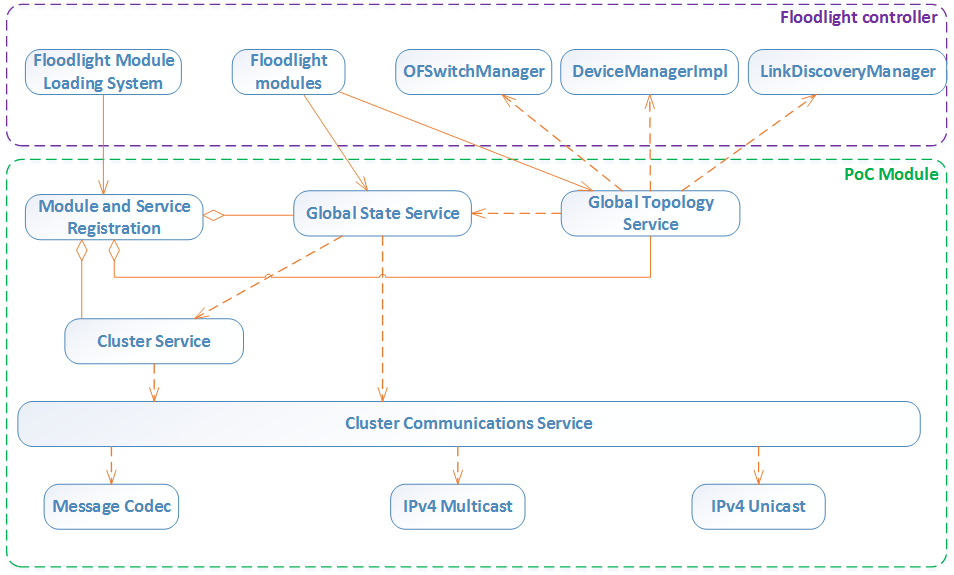
\includegraphics[scale=0.65]{amorphous_block_diagram}
	\caption{Proof of concept implementation high level block diagram}
	\label{fig:amorphous_block_diagram}
\end{figure}
%

%TODO: APIs exposed
%NOTE: Instance health and Join cluster messages merged for performance optimization
%TODO: IPv4 Multicast vs Unicast (why and when)

%TODO Overall workflow

%
\section{Request Router}
\label{section:request-router}
%TODO: Linux LVS
%TODO: DSR
%TODO: Anycast mechanism: BGP ECMP (Quagga) + Loopback on Controllers + disable RPF on core routers
%TODO: Request Router component (Multicast integration)
